%============================================================
% CH1 · PATTERN 3 — EXERCISES, HINTS, ANSWERS
%============================================================
\subsection{Pattern 3: Exercises and Going Further}
\label{ssec:ch1-p3-ex}

\begin{patternbox}{Pattern 3 Summary Card}
\begin{tabularx}{\linewidth}{@{}>{\bfseries}l X@{}}
Model & open cell = vertex; two open cells sharing a side = edge (8 directions if corners count); the graph stays implicit \\
Algorithm & scan in row-major order; an unvisited open cell starts a flood fill (stack, queue or recursion) that marks its whole component \\
Answers & \#fills = \#components; pops per fill = size; sum of values per fill = volume \\
Cost & $\bigO{nm}$ time and memory; $|E| \le 2nm$ \\
Top traps & bounds after access; marking on pop; recursion depth $nm$; 4 vs 8 neighbours; \texttt{r*n+c}; recolouring with the same colour \\
\end{tabularx}
\end{patternbox}

\exlegend
\begin{enumerate}[leftmargin=*, label=\textbf{E3.\arabic*}, itemsep=6pt]
    \item \exeasy\ \pconcept \exprob{Island Perimeter}{LeetCode 463}{https://leetcode.com/problems/island-perimeter/}\ \lc{Easy}. A $0/1$ grid ($\le 100\times100$) contains exactly one island (4-connected, no lakes inside). Return the length of its boundary, every cell being a $1\times1$ square. (\texttt{[[0,1,0,0],[1,1,1,0],[0,1,0,0],[1,1,0,0]]} $\to 16$.)
    \item \exeasy\ \ptricky \exprob{Flood Fill}{LeetCode 733}{https://leetcode.com/problems/flood-fill/}\ \lc{Easy}. Recolour the 4-connected region of pixels that have the same colour as \texttt{image[sr][sc]} and contain it, with a new \texttt{color}; return the image. (\texttt{[[1,1,1],[1,1,0],[1,0,1]]}, $(1,1)$, $2$ $\to$ \texttt{[[2,2,2],[2,2,0],[2,0,1]]}.)
    \item \exeasy\ \pconcept \cf{1100}\\exprob{The Lakes}{Codeforces 1829E}{https://codeforces.com/problemset/problem/1829/E}. $t$ test cases; each is an $n\times m$ grid of depths $0 \le a_{ij} \le 1000$ with $\sum nm \le 10^6$. A lake is a 4-connected component of cells with positive depth, its volume is the sum of the depths. Print the largest volume (0 if there is no lake).
    \item \exmedium\ \ptricky \exprob{Count Sub Islands}{LeetCode 1905}{https://leetcode.com/problems/count-sub-islands/}\ \lc{Medium}. Two $0/1$ grids of the same size ($\le 500\times500$). An island of \texttt{grid2} is a \emph{sub-island} if every one of its cells is land in \texttt{grid1}. Count the sub-islands.
    \item \exhard\ \pclassic \exprob{Making A Large Island}{LeetCode 827}{https://leetcode.com/problems/making-a-large-island/}\ \lc{Hard}. In an $n\times n$ $0/1$ grid ($n \le 500$) you may change at most one $0$ into $1$. Return the largest possible island area. (\texttt{[[1,0],[0,1]]} $\to 3$.)
    \item \exmedium\ \pconcept \exown{Four or eight neighbours?} For the grid below, count the islands under 4-connectivity and under 8-connectivity, by hand, then with code. Which single direction-array change turns one program into the other?
    \begin{center}\ttfamily 1 0 0 1 \quad / \quad 0 1 1 0 \quad / \quad 0 1 0 0 \quad / \quad 1 0 0 1\end{center}
    \item \exmedium\ \precent \exprob{Count Islands With Total Value Divisible by K}{LeetCode 3619}{https://leetcode.com/problems/count-islands-with-total-value-divisible-by-k/}\ \lc{Medium}. An $m\times n$ grid of values $0 \le v \le 10^6$ ($mn \le 10^5$); an island is a 4-connected group of positive cells, and its total value is the sum of its cells. Count the islands whose total value is divisible by $k$ ($1 \le k \le 10^6$).
\end{enumerate}

\subsubsection*{Hints}
\begin{enumerate}[leftmargin=*, label=\textbf{E3.\arabic*}]
    \item Every land cell brings 4 sides; every edge between two land cells hides 2 of them. No traversal needed.
    \item ``Visited'' is ``already has the new colour'' --- but what if the new colour equals the old one?
    \item Problem 1.3.2 with the depth added instead of 1. Watch the total size of all tests and the maximum sum ($10^6\cdot1000$).
    \item Fill each island of \texttt{grid2} \emph{completely}, even after you have found a cell that is water in \texttt{grid1}.
    \item Paint each island with its own id and remember its area. A $0$ cell touches at most 4 islands --- but maybe the same island twice.
    \item Draw the corner contacts. The 4-direction array is a prefix of the 8-direction array.
    \item The Lakes (E3.3) again, but you test each sum instead of taking the maximum. How large can one sum get?
\end{enumerate}

\subsubsection*{Answers}

\begin{solutionbox}[E3.1 Island Perimeter]
Count land cells $L$ and land--land edges $S$ (look only down and right, so each edge is counted once). Perimeter $= 4L - 2S$.
\begin{lstlisting}[style=cpp]
#include <bits/stdc++.h>
using namespace std;

class Solution {
public:
    int islandPerimeter(vector<vector<int>>& grid) {
        int R = grid.size(), C = grid[0].size(), land = 0, shared = 0;
        for (int r = 0; r < R; r++)
            for (int c = 0; c < C; c++) {
                if (grid[r][c] != 1) continue;
                land++;
                if (r + 1 < R && grid[r + 1][c] == 1) shared++;   // edge below
                if (c + 1 < C && grid[r][c + 1] == 1) shared++;   // edge right
            }
        return 4 * land - 2 * shared;
    }
};
\end{lstlisting}
\begin{center}
\begin{tikzpicture}
    \def\gIpIIIs{0.55}
    \gIpIIIgrid{waww,aaaw,waww,aaww}
    \node[note, anchor=west, text width=6.5cm, align=left] at (2.3,-0.8) {Example 1: $L = 7$ land cells, $S = 6$ shared edges ($(0,1){-}(1,1)$, $(1,0){-}(1,1)$, $(1,1){-}(1,2)$, $(1,1){-}(2,1)$, $(2,1){-}(3,1)$, $(3,0){-}(3,1)$): $28 - 12 = 16$. The other examples give 4 and 4.};
\end{tikzpicture}
\end{center}
This is a pure counting argument on the grid graph (Pattern 1 thinking): no fill at all, because the island is the only one. The ``no lakes'' promise matters: with a lake, its shore would also count as perimeter --- and the formula would \emph{still} give the total boundary length.
\end{solutionbox}

\begin{solutionbox}[E3.2 Flood Fill]
The region is the component of $(sr,sc)$ in the graph ``same-coloured neighbours''. Recolour while filling; a pixel that already has the new colour is never entered again. If the old colour equals the new one, return at once --- otherwise the recursion would bounce between two pixels forever.
\begin{lstlisting}[style=cpp]
#include <bits/stdc++.h>
using namespace std;

class Solution {
    void fill(vector<vector<int>>& img, int r, int c, int from, int to) {
        if (r < 0 || r >= (int)img.size() || c < 0 || c >= (int)img[0].size()) return;
        if (img[r][c] != from) return;
        img[r][c] = to;
        fill(img, r - 1, c, from, to); fill(img, r + 1, c, from, to);
        fill(img, r, c - 1, from, to); fill(img, r, c + 1, from, to);
    }
public:
    vector<vector<int>> floodFill(vector<vector<int>>& image, int sr, int sc, int color) {
        int from = image[sr][sc];
        if (from != color) fill(image, sr, sc, from, color);   // equal colours: nothing to do
        return image;
    }
};
\end{lstlisting}
Example 1 gives \texttt{[[2,2,2],[2,2,0],[2,0,1]]} (the bottom-right 1 touches the region only at a corner); Example 2 (\texttt{color} equal to the old colour 0) returns the image unchanged. The grid is at most $50\times50$, so recursion is safe. Checked against a BFS recolouring on 5000 random images.
\end{solutionbox}

\begin{solutionbox}[E3.3 The Lakes]
Scan; a positive cell starts a fill that adds up the depths of the cells it reaches and sets them to 0. With $\sum nm \le 10^6$ use an explicit stack (an open $1000\times1000$ lake would recurse $10^6$ deep) and allocate the grid per test. The largest volume is at most $10^6 \cdot 1000 = 10^9$, which still fits in \texttt{int}; \texttt{long long} costs nothing and removes the doubt.
\begin{lstlisting}[style=cpp]
#include <bits/stdc++.h>
using namespace std;

int main() {
    ios::sync_with_stdio(false);
    cin.tie(nullptr);
    int t;
    cin >> t;
    while (t--) {
        int n, m;
        cin >> n >> m;
        vector<vector<int>> a(n, vector<int>(m));
        for (auto& row : a) for (auto& x : row) cin >> x;
        const int dr[4] = {-1, 1, 0, 0}, dc[4] = {0, 0, -1, 1};
        long long best = 0;                        // no lake at all -> 0
        vector<int> st;
        for (int r = 0; r < n; r++)
            for (int c = 0; c < m; c++) {
                if (a[r][c] == 0) continue;
                long long volume = 0;
                st.push_back(r * m + c);
                volume += a[r][c];
                a[r][c] = 0;                       // visited = depth set to 0
                while (!st.empty()) {
                    int x = st.back() / m, y = st.back() % m;
                    st.pop_back();
                    for (int d = 0; d < 4; d++) {
                        int nx = x + dr[d], ny = y + dc[d];
                        if (nx < 0 || nx >= n || ny < 0 || ny >= m || a[nx][ny] == 0) continue;
                        volume += a[nx][ny];
                        a[nx][ny] = 0;
                        st.push_back(nx * m + ny);
                    }
                }
                best = max(best, volume);
            }
        cout << best << "\n";
    }
}
\end{lstlisting}
On the five official samples the program prints 10, 0, 7, 16, 21. In the fourth sample the ring of 1s around the 5 is one lake of volume 16, and the 5 is a separate lake (its neighbours are 0): $\max(16,5) = 16$. In the fifth the 4 touches the ring, so everything is one lake: $17 + 4 = 21$.
\end{solutionbox}

\begin{solutionbox}[E3.4 Count Sub Islands]
Fill every island of \texttt{grid2}; while filling, AND a flag ``this cell is land in \texttt{grid1}''. Do \textbf{not} stop the fill when the flag becomes false: the rest of the island must still be sunk, otherwise its remaining cells would later be counted as a separate (wrong) island.
\begin{lstlisting}[style=cpp]
#include <bits/stdc++.h>
using namespace std;

class Solution {
public:
    int countSubIslands(vector<vector<int>>& grid1, vector<vector<int>>& grid2) {
        int R = grid2.size(), C = grid2[0].size(), cnt = 0;
        const int dr[4] = {-1, 1, 0, 0}, dc[4] = {0, 0, -1, 1};
        for (int r = 0; r < R; r++)
            for (int c = 0; c < C; c++) {
                if (grid2[r][c] != 1) continue;
                bool inside = true;                    // every cell so far is land in grid1
                vector<pair<int,int>> st(1, make_pair(r, c));
                grid2[r][c] = 0;                       // sink grid2's island as we go
                while (!st.empty()) {
                    int x = st.back().first, y = st.back().second;
                    st.pop_back();
                    if (grid1[x][y] == 0) inside = false;   // do NOT stop: finish the fill
                    for (int d = 0; d < 4; d++) {
                        int nx = x + dr[d], ny = y + dc[d];
                        if (nx < 0 || nx >= R || ny < 0 || ny >= C || grid2[nx][ny] != 1) continue;
                        grid2[nx][ny] = 0;
                        st.push_back(make_pair(nx, ny));
                    }
                }
                if (inside) cnt++;
            }
        return cnt;
    }
};
\end{lstlisting}
Why is ``all cells are land in \texttt{grid1}'' enough --- must they lie in the \emph{same} island of \texttt{grid1}? Yes, automatically: the island of \texttt{grid2} is connected, and if all its cells are land in \texttt{grid1}, the same paths connect them in \texttt{grid1}. Examples: 3 and 2. Checked against a brute force (label both grids, compare label sets) on 5000 random pairs.
\end{solutionbox}

\begin{solutionbox}[E3.5 Making A Large Island]
\textbf{Step 1:} paint every island with its own id $2, 3, \dots$ (ids 0 and 1 are taken) and store \texttt{area[id]}. \textbf{Step 2:} for every $0$ cell, collect the \emph{distinct} ids among its 4 neighbours; flipping it gives $1 + \sum$ their areas. The answer is the maximum of these values and of the largest existing island (the grid may contain no $0$ at all).
\begin{lstlisting}[style=cpp]
#include <bits/stdc++.h>
using namespace std;

class Solution {
public:
    int largestIsland(vector<vector<int>>& grid) {
        int n = grid.size();
        const int dr[4] = {-1, 1, 0, 0}, dc[4] = {0, 0, -1, 1};
        vector<int> area(2, 0);                    // area[id] for island ids 2, 3, ...
        for (int r = 0; r < n; r++)
            for (int c = 0; c < n; c++) {
                if (grid[r][c] != 1) continue;
                int id = area.size(), a = 0;       // paint this island with colour id
                vector<int> st(1, r * n + c);
                grid[r][c] = id;
                while (!st.empty()) {
                    int x = st.back() / n, y = st.back() % n;
                    st.pop_back();
                    a++;
                    for (int d = 0; d < 4; d++) {
                        int nx = x + dr[d], ny = y + dc[d];
                        if (nx < 0 || nx >= n || ny < 0 || ny >= n || grid[nx][ny] != 1) continue;
                        grid[nx][ny] = id;
                        st.push_back(nx * n + ny);
                    }
                }
                area.push_back(a);
            }
        int best = 0;
        for (size_t id = 2; id < area.size(); id++) best = max(best, area[id]);   // no flip needed
        for (int r = 0; r < n; r++)
            for (int c = 0; c < n; c++) {
                if (grid[r][c] != 0) continue;
                int ids[4], k = 0, total = 1;      // the flipped cell itself
                for (int d = 0; d < 4; d++) {
                    int nr = r + dr[d], nc = c + dc[d];
                    if (nr < 0 || nr >= n || nc < 0 || nc >= n || grid[nr][nc] == 0) continue;
                    int id = grid[nr][nc];
                    bool dup = false;              // the same island may touch twice
                    for (int j = 0; j < k; j++) if (ids[j] == id) dup = true;
                    if (!dup) { ids[k++] = id; total += area[id]; }
                }
                best = max(best, total);
            }
        return best;
    }
};
\end{lstlisting}
\begin{center}
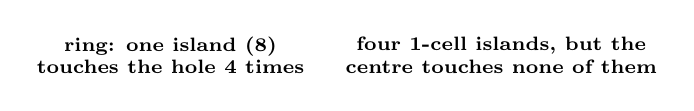
\begin{tikzpicture}
    \def\gIpIIIs{0.55}
    \begin{scope}
        \gIpIIIgrid{aaa,axa,aaa}
        \node[font=\scriptsize\bfseries, align=center] at (0.55,-1.65) {ring: one island (8)\\touches the hole 4 times};
    \end{scope}
    \begin{scope}[xshift=4.2cm]
        \gIpIIIgrid{awb,wxw,cwd}
        \node[font=\scriptsize\bfseries, align=center] at (0.55,-1.65) {four 1-cell islands, but the\\centre touches none of them};
    \end{scope}
\end{tikzpicture}
\end{center}
The ring ($3\times3$ of 1s with a 0 in the middle) must give $1 + 8 = 9$, not $1 + 4\cdot8 = 33$ --- that is what the \texttt{dup} test is for. In the second picture the centre has only water neighbours, so the best flip is next to a corner island: $1+1+1 = 3$. Official examples: 3, 4, 4. All verified against a brute force that tries every flip and recomputes the largest island, on 5000 random grids. Total $\bigO{n^2}$.
\end{solutionbox}

\begin{solutionbox}[E3.6 Four or eight neighbours?]
\begin{center}
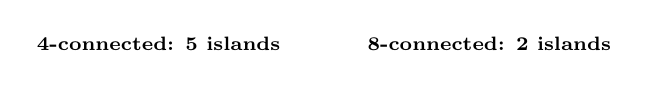
\begin{tikzpicture}
    \def\gIpIIIs{0.55}
    \begin{scope}
        \gIpIIIgrid{AwwB,wCCw,wCww,Dwwe}
        \gIpIIIat{3}{3}{E}
        \node[font=\scriptsize\bfseries] at (0.82,-2.4) {4-connected: 5 islands};
    \end{scope}
    \begin{scope}[xshift=4.2cm]
        \gIpIIIgrid{Awwa,wAAw,wAww,awwb}
        \gIpIIIat{0}{3}{A}\gIpIIIat{3}{0}{A}\gIpIIIat{3}{3}{B}
        \node[font=\scriptsize\bfseries] at (0.82,-2.4) {8-connected: 2 islands};
    \end{scope}
\end{tikzpicture}
\end{center}
Under 4-connectivity: the three middle cells form one island and the four corners are alone: \textbf{5}. Under 8-connectivity the corners $(0,0)$, $(0,3)$ and $(3,0)$ each touch the middle island diagonally, but $(3,3)$ touches only water: \textbf{2}. (Our program prints 5 and 2.) With the arrays
\texttt{dr = \{-1,1,0,0,-1,-1,1,1\}}, \texttt{dc = \{0,0,-1,1,-1,1,-1,1\}}, the loop \texttt{for (d = 0; d < K; d++)} gives 4-connectivity for $K = 4$ and 8-connectivity for $K = 8$ --- one number is the whole difference.
\end{solutionbox}

\begin{solutionbox}[E3.7 Count Islands With Total Value Divisible by K]
Scan; every positive cell starts a fill that adds up the values and sets the cells to $0$; after the fill, test \texttt{sum \% k == 0}. The trap is the size of the sum: one island can hold $10^5$ cells of value $10^6$, a total of $10^{11}$, which overflows a 32-bit \texttt{int}. Use \texttt{long long} (or keep only \texttt{sum \% k}). The fill uses an explicit stack, because an island can have $10^5$ cells.
\begin{lstlisting}[style=cpp]
#include <bits/stdc++.h>
using namespace std;

class Solution {
public:
    int countIslands(vector<vector<int>>& grid, int k) {
        int R = grid.size(), C = grid[0].size(), cnt = 0;
        const int dr[4] = {-1, 1, 0, 0}, dc[4] = {0, 0, -1, 1};
        vector<int> st;
        for (int r = 0; r < R; r++)
            for (int c = 0; c < C; c++) {
                if (grid[r][c] == 0) continue;
                long long sum = grid[r][c];            // up to 1e5 * 1e6: needs 64 bits
                grid[r][c] = 0;                        // visited = value set to 0
                st.push_back(r * C + c);
                while (!st.empty()) {
                    int x = st.back() / C, y = st.back() % C;
                    st.pop_back();
                    for (int d = 0; d < 4; d++) {
                        int nx = x + dr[d], ny = y + dc[d];
                        if (nx < 0 || nx >= R || ny < 0 || ny >= C || grid[nx][ny] == 0) continue;
                        sum += grid[nx][ny];
                        grid[nx][ny] = 0;
                        st.push_back(nx * C + ny);
                    }
                }
                if (sum % k == 0) cnt++;
            }
        return cnt;
    }
};
\end{lstlisting}
Example 1 ($k = 5$) has four islands with sums $2+1+5 = 8$, $5$, $1+1+4+7+2 = 15$ and $8$; two of them are divisible by 5, so the answer is \textbf{2}. In Example 2 ($k = 3$) there are six single cells of value 3, all divisible: \textbf{6}. Checked against a brute force (DSU labels, then the sum per label) on 5000 random grids, and on one $1\times10^5$ island of $10^6$s (sum $10^{11}$).
\end{solutionbox}
